%%% Template originaly created by Karol Kozioł (mail@karol-koziol.net) and modified for ShareLaTeX use

% \documentclass[a4paper,11pt]{article}
\documentclass[a4paper,11pt]{article}

\usepackage[english]{babel}
\usepackage{hyperref}
\usepackage[T1]{fontenc}
\usepackage[utf8]{inputenc}
\usepackage{graphicx}
\usepackage{xcolor}
\usepackage{xcolor}
\usepackage[linesnumbered, boxed,ruled,vlined]{algorithm2e}
\usepackage{algpseudocode}

\renewcommand\familydefault{\sfdefault}
\usepackage{tgheros}
% \usepackage[defaultmono]{droidmono}

\usepackage{amsmath,amssymb,amsthm,textcomp}
\usepackage{enumerate}
\usepackage{multicol}
\usepackage{tikz}

\usepackage{geometry}
\geometry{left=10mm,right=15mm,%
bindingoffset=5mm, top=15mm, bottom=20mm}


\linespread{1.3}

\newcommand{\linia}{\rule{\linewidth}{0.5pt}}

% custom theorems if needed
\newtheoremstyle{mytheor}
{1ex}{1ex}{\normalfont}{0pt}{\scshape}{.}{1ex}
{{\thmname{#1 }}{\thmnumber{#2}}{\thmnote{ (#3)}}}

\theoremstyle{mytheor}
\newtheorem{defi}{Definition}

% my own titles
\makeatletter
\renewcommand{\maketitle}{
\begin{center}
\vspace{2ex}
{\huge \textsc{\@title}}
\vspace{1ex}
\\
\begin{center}
\@author
\end{center}
\end{center}
}
\makeatother
%%%

% custom footers and headers
\usepackage{fancyhdr}
\pagestyle{fancy}
\lhead{}
\chead{}
\rhead{}
% \lfoot{Assignment \textnumero{} 1}
% \cfoot{}
\cfoot{Page \thepage}
\renewcommand{\headrulewidth}{0pt}
\renewcommand{\footrulewidth}{0pt}
%

% code listing settings
\usepackage{listings}
\lstset{
language=Python,
basicstyle=\ttfamily\small,
aboveskip={1.0\baselineskip},
belowskip={1.0\baselineskip},
columns=fixed,
extendedchars=true,
breaklines=true,
tabsize=4,
prebreak=\raisebox{0ex}[0ex][0ex]{\ensuremath{\hookleftarrow}},
frame=lines,
showtabs=false,
showspaces=false,
showstringspaces=false,
keywordstyle=\color[rgb]{0.627,0.126,0.941},
commentstyle=\color[rgb]{0.133,0.545,0.133},
stringstyle=\color[rgb]{01,0,0},
numbers=left,
numberstyle=\small,
stepnumber=1,
numbersep=10pt,
captionpos=t,
escapeinside={\%*}{*)}
}

%%%----------%%%----------%%%----------%%%----------%%%
\frenchspacing
%%% ---- CUSTOM SETTINGS BY OLU --- %%%
\setlength\parindent{0pt}


\begin{document}

\title{Multi-Agent Systems Final Report}

\author{Samuel Meyer (5648122) \and Sorin Dragan (6884393) \and Markos Polos (6943721) \and Olusanmi Hundogan (6883273) \and Group 10}

\maketitle
\hline

\subsection{Introduction}

\subsection{THINGS THAT NEED TO BE INCORPORATED}
- A high-level description of the agent and its structure, \textbf{including the main Java methods (mention these explicitly!)} used in the negotiating agent that have been implemented in the source
code. This includes detail of any changes that were made to the original agent design and a motivation for these;\newline

– An explanation of the negotiation strategy, decision function for accepting offers, estimators
for preference uncertainty, any important preparatory steps, learning techniques, and heuristics
that the agent uses to decide what to do next;\newline

– A section documenting the strong and weak points of your agent, the tests you performed
to analyze (and improve) the negotiation strength of your agent. You must include scores of
various tests over multiple sessions that you performed. Describe how you set up the testing
situation and how you used the results to modify your agent, and motivate why you choose
these testing methods/metrics/graphs \textbf{Sorin parameter tweak statistics?};\newline

– Answers to the questions posed in the assignment;\newline

– A final conclusion written by the group coordinator, in which the coordinator discusses a summary of the experience of the team with regards to writing the report and building the negotiating agent, and a summary of who performed which tasks.\newline

- The source code should contain explanatory comments that will allow third parties not involved
in programming the code to understand it. A clear explanation of a method must be provided at
the beginning of important methods. Parts of the code that are not self-explaining should receive
additional documentation. Please incorporate enough information in comments in the code to ensure
this. Finally, make sure that you have removed all debug printouts from your code and that your
agent does not flood the ’System.out’ channel \newline

\section{Agent Implementation}
\subsection{Uncertainty Utility Estimation}
Based on a set of preferences, an agent in a negotiation setting generally attempts to maximize a personal utility value based on these preferences. However, the agent doesn't always know these preferences, so it cannot be certain of the utility values of bids that it proposes or receives from other agents. Based on the negotiation setting, there is some information that is available to the agent under preference uncertainty. Out of all possible bids that can be made within a domain, the agent receives a ranked subset of bids. Each bid in this ranking has a higher utility than the bid before it. The agent also knows the exact utility of the best and worst bids in the ranking. Using this information, it is possible to estimate the utilities of any bid. \newline

The approach taken is an adjustment to that taken in the paper [reference]. In this approach, the problem of estimating the utility function is translated to a linear programming problem. Each issue value has its own associated utility that is weighted based on issue preferences:

\begin{center}
    $\phi_i(\omega_i) = w_i · v_i(\omega_i)$ \\
\end{center}

With issue i, bid $\omega$, issue weight w, and utility function v. The goal is to estimate $\phi$ for each issue to produce a linear additive function $\sum_{i=1}^{m}\phi_i(\omega_i)$ that estimates the utility of a bid. Given the ranked bids are ordered from least preferred to most preferred bids, the utility of one bid is lower than that of the next bid for each adjacent pair in this ranking. Thus, the utility of the preferred bid subtracted from the utility of the less preferred bid in a pair must be greater than zero. For each adjacent pair of bids in the given ranking, this is added as a constraint. In our implementation, bids are 1-hot encoded for each issue, and a pairwise comparison is the subtraction of one encoding from another. For each comparison, a slack variable $z_{o,o'}$ is introduced, with $o$ and $o'$ consecutive bids in the ranking. To make sure that each pairwise comparison will result in a value greater than zero given the estimates of $\phi$, the contribution of the slack variables should ideally be zero. The function to be minimized through linear programming is then the sum of these slack variables. As base constraints, each estimate of $\phi_i$ and $z_{o,o'}$ should be greater than or equal to zero. With this optimization target and set of constraints, the optimization leads to the trivial solution. To solve this, the original approach adds the constraint that the most preferred bid in the ranking must have a utility of 1. In the negotiation setting for our agent, we get the exact utilities of the worst and best bid of the received ranking, so we added these bids and their values as additional constraints. Since the bids between the most and least preferred bids must also have utilities values between those of the most and least preferred bids, these conditions were added to constrain the problem even further. With these constraints, the simplex algorithm was then used to solve the linear programming problem. \textbf{(SHOULD WE ADD DATA SO CAN CLAIM THAT OUR ADDITIONS MAKE FOR BETTER RESULTS? - OR MAYBE WE CAN EXPLAIN HOW THIS MIGHT MAKE US BETTER THAN OTHER AGENTS IN THE SECTION FOR TESTING OF PREFERENCE UNCERTAINTY)}


\subsection{Acceptance Strategy}
The acceptance strategy of our agent consists of three main ideas. The first is the time-based influence $\mathcal{E} \in (0,1)$. When deciding whether to accept an opponent bid $bid_o^t$ at time $t$, its utility is compared to that of the next bid our agent will make $bid_a^{t+1}$. The opponent bid will pass this part of the acceptance strategy if its utility is greater than that of our agent's next bid. To take time into account, a time factor $\mathcal{E}$ is added to the utility of the opponent bid to make condition $u(bid_a^{t+1}) > u(bid_o^t) + \mathcal{E}$. This increases the odds of reaching an agreement by the end of the negotiation. The value of $\mathcal{E}$ is calculated with $x=\frac{time step}{deadline}$ as function $f(x)=\frac{0.02}{1.05 - x}$. The value of $\mathcal{E}$ starts close to 0, slowly increases over the course of the negotiation, and near the final time step quickly reaches a value of approximately 0.5. Thus, as long as the opponent bid gives us a utility of at least 0.5 by the end, it is guaranteed to be accepted. If a bid has not been rejected as a result of the above, the second idea comes into play – the use of the opponent bidding history H. If the bidding history of an opponent has a bid with a higher utility for our agent than its current one, the bid is rejected and the next bid our agent proposes will be the past bid that was found in H. Thus, if facing an opponent that backs away from a concession, our agent attempts to hold them to that concession. After re-proposing the opponent bid, this bid will not be reconsidered as the best opponent bid again. This prevents the acceptance strategy from getting stuck re-proposing the same bid when an opponent does not ever move back towards the earlier concession. If the first two ideas do not lead to a rejection, the opponent bid is assessed based on the final notion. The final component is based on our agent’s prediction of the next opponent bid. 
If our agent predicts that upon rejection, the next opponent bid will have a higher utility for our agent than the current bid, the current bid is rejected. If the opponent bid was not rejected through all three components, the bid is accepted. The estimation of the opponent's bidding strategy will be discussed in \autoref{sec:OBS}. The full process is displayed in \autoref{alg:IR}:\\

\begin{algorithm}[H]
\SetAlgoNoEnd\SetAlgoNoLine
\SetKwIF{If}{ElseIf}{Else}{if}{:}{else if}{else:}{}%
 %\KwData{What does}
 %\KwResult{This look like?}
%\TitleOfAlgo{}
\SetAlgoCaptionLayout{textbf}
\eIf{$u(bid_a^{t+1}) \leq u(bid_o^t) + \mathcal{E}$}{
    \uIf{$\exists t' \in H$ such that $u(bid_o^{t}) < u(bid_o^{t'})$}
        {Reject bid, propose $bid_o^{t'}$ as next bid $bid_a^{t+1}$\\
        Pop $bid_o^{t'}$ from H}
    \uElseIf{$u(bid_o^{t}) \leq$ predicted $u(bid_{o}^{t+1})$}
        {Reject}
    {Accept bid}
    }
{Reject bid}
\caption{Acceptance Strategy}\label{alg:IR}
\end{algorithm}

\subsection{Opponent Bidding Strategy Model}
\label{sec:OBS}
A core component of MCTS is the simulation of various session rollouts. However, learning the opponents behaviour which can suddenly change is a non-trivial moving target problem.\cite{Baarslag2016} Baarslag et. al mentions several methods for learning the opponents bidding strategy.\cite{Baarslag2016} Generally divided into regression analysis and time series analysis, the latter do not assume any underlying decision function. In particular, the signal processing method Gaussian Process Regression has multiple advantages. First, it does not require pretraining. Second, Gaussian processes can be used for classification problems. Third, it can predict moving targets. The aim of using GPR in this context is to estimate the opponents next expected bid $y_*$ given an unobserved $x_*$ and a history of observations ($X,Y$). The input $X$ represents the history of both, the opponents and the agents, one-hot encoded bids. $Y$ is the agent's utility of the following bid. Equations 1 and 2 describe the calculation.\cite{Buron_Guessoum_Ductor_2019}

\begin{align}
    \label{eq:GPR}
    K &= \begin{bmatrix}
    k(x_1,x_1)&\cdots &k(x_n,x_1) \\
    \vdots & \ddots & \vdots\\
    k(x_1,x_n)&\cdots &k(x_n,x_n)
    \end{bmatrix} & K_* &= [k(x_*,x_1), \cdots, k(x_*,x_n)]\\
    y_* &= K_*K^{-1}Y &\sigma_*^2 &= K_{**} - K_* K^{-1} K_*^T
\end{align}

Equation (1) describes the proximity in terms of covariance matrices $K$ and $K_*$ for features $X$ and $x_*$. $K$ refers to the covariance matrix within the set of $X$, whereas $K_*$ describes the covariance vector between $x_*$ and $X$. $k(a,b)$ denotes a kernel function as proximity measure. With $Y$ being the previous utilities and $y_*$ the expected utility, we can calculate $\mathbb{E}[y_*|K_*,K,Y]$ and its variance $\sigma_*^2$. By assuming that each $X$ form a multivariate Gaussian, equations in (2) follow. Afterwards, $y_*$ and $\sigma_*^2$ be used to sample a random utility and generate a bid near that utility.

\subsection{Agent Bidding Strategy}
 The first bid offered by the agent is separate by the strategy and will always be the one that will result in the highest possible utility. The bidding strategy relays on the use of a Monte Carlo Search Tree (MCTS) which was also proposed by Buron et al. (CITE HERE) This method proved to be useful in games with large branching factors, like Go. (CITE HERE) A negotiation can also be seen as a game with a large branching factor in which an action is represented by placing a bid. Each node of the MCTS stores information about the score and number of visits together with a bid which is going to be made if the node will be chosen. The MCTS algorithm consists of the 4 phases presented in Figure 1, namely selection, expansion, simulation (also referred as the rollout), and backpropagation. 
\begin{figure}[h!]
  \centering
  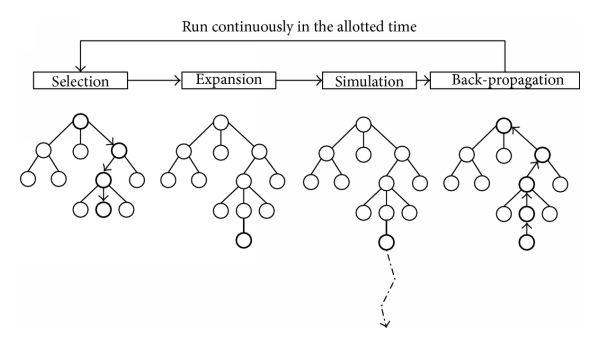
\includegraphics[width=0.5\linewidth]{report2/mcts_pic.png}
  \caption{The steps of the Monte Carlo Tree Search algorithm.\cite{MTCS_tree_pic}}
  \label{fig:preferences}
\end{figure}

In the \textbf{selection} phase, the algorithm selects the best leaf node. This is done by choosing the best child node at each level of the tree based on the UCB1 formula (WRITE THE MATH FORMULA HERE). The \textbf{expansion} happens only when the number of visits of the node in question is greater or equal the the number of children it possess. Expanding a node creates 3 new empty nodes and fills them with a random bid within a lower-bound - upper-bound range. The upper-bound is always set to the maximum utility of 1.0. The lower-bound decreases while being dependant on time. It will start at 1.0 and linearly decrease towards a fraction of 1.0. In the tests we ran, the minimum possible that could be reached by the lower-bound at the end of the negotiation was 0.75. We also considered a sigmoid related decrease, but the linear one seemed to yield better results in practice. The \textbf{rollout} phase is simulating a limited number of steps of the rest of the negotiation based on the similar random bids within a range on the agent's side and the bids predicted by \textbf{Opponent Bidding Strategy Model} (OBSM) on the opponent's side. The simulation ends either when the \textbf{Acceptance Strategy} of the agent accepts a bid generated by the OBSM or when a previously set maximum depth is reached. During the simulation a discounted average of the utilities resulted from the OBSM bids is calculated. This average represents the score that will be propagated up by the \textbf{backpropagation} step. During the backpropagation, each node will be updated the score, as an additive average, and the number of visits. These steps are ran multiple times each negotiation turn in order to facilitate the construction of the tree. After the tree is constructed, the strategy will choose the child of the root with the highest score and it will offer bid saved in that node. The chosen node will be the root of the tree at the next negotiation turn. The proposed bids are not only highly dependent on the performance of the OBSM but they are also dependant on an element of chance, as the bids are randomly selected within a given range. This also means that, as the game evolves and lower-bound decreases, future bids can have higher values than older ones. However, the overall bidding will follow a linear form of conceding. \\
\\
TODO: write about parameters, t, freq, depth. The freq seems to be the most important one: the more we explore the space the better the results; t/10 to strict yields worse results.
\\
Note on improvements part: tweaking conceding based on the behaviour of the opponent; integrate the opponent preference model to constraint the random bidding to aim for the Pareto line;

\section{Quantifying Agent Performance}
Most of the tests were conducted on the party domain with profile 1 and 2. From several tournament configurations, that the agent performs better in a tournament with higher numbers of participants. However, 
we tested our agent under uncertainty in a tournament that had NiceTitForTat, RandomDancer, KLH HardHeaded, IAMhaggler, and the Negotiator as other participants. By choosing these agents we aimed at a balanced mix of strong boulware, conceder, random and mixed type strategies. In the following they are referred to as standard opponents. The final ranking was calculated using the sum of utility along all the negotiations. In the party domain, the agent obtained a total utility of 7.67 across 10 games with an average time of agreement of 56.6 rounds and an average distance from the Pareto line of 0.13. The agent reached an agreement in 90\% of the games.


\subsection{The Agent Under Uncertainty}
 HardHeaded came 1st proving that a more Boulware strategy is beneficial in small tournaments. In the case of \textbf{uncertainty 10}, we finished last in the tournament as the sum of utility (5.13) and the sum of utility perceived by the agent (9.10) were too different. (MAYBE RUN THIS AGAIN OR WHAT IS THE DEAL HERE?). Under \textbf{uncertainty 20} and \textbf{uncertainty 50}, the agent won the tournament with 0.58, respectively 0.79 average utility per negotiation. In the uncertainty 20 case, the agent reached an agreement in only 70\% of cases and had an 0.41 average distance from the Pareto frontier. Under uncertainty 50, the perceived sum of utilities had a deviation of only 0.09 from the actual sum of utility. An agreement was always reached and the average distance from the Pareto frontier was 0.07. The robustness (WHAT IS THIS?) was 0.08 and the difference from the second place was 0.75.

\begin{table}[htb]
\centering
\begin{tabular}{l||lllll}
\hline
%  &\multicolumn{4}{c}{}                   \\ \hline\hline
                & Party U10         & Party U20              & Party U50      \\ \hline\hline
TheNegotiator   & \textbf{7.18}  & 7.57 & 8.60  &  & 8.21   \\ 
NiceTitForTat   & 6.95  & 7.25 & \textbf{8.94}  &  & 8.62   \\ 
RandomDance     & 5.42  & 7.17 & 8.49  &  & 8.84 \\ 
IAMhaggler2012  & 5.88  & 6.49 & 7.64  &  & 8.59  \\ 
KLH             & 5.72  & 7.56 & 8.49  &  & \textbf{9.63}   \\ 
CarlosBoaParty  & 7.06  & \textbf{7.67} & 8.63  &  & 9.42   \\ 
\end{tabular}
\caption{Sum of utilities with varying domains}
\end{table}

\subsection{The Agent Under Different Domains}
We tested the agent under different domains against the standard opponents in form of tournaments. The domains were: the SmartGrid and Party domain as simple domains; the Laptop domain with the buyer being uncertain; the pie domain with one issue yielding many values; and domain 16 having a large amount of issue with at 2 values.

\begin{table}[htb]
\centering
\begin{tabular}{l||lllll}
\hline
%  &\multicolumn{4}{c}{}                   \\ \hline\hline
                & SmartGrid         & Party              & Laptop             & Pie & Domain16      \\ \hline\hline
TheNegotiator   & \textbf{7.18}  & 7.57 & 8.60  &  & 8.21   \\ 
NiceTitForTat   & 6.95  & 7.25 & \textbf{8.94}  &  & 8.62   \\ 
RandomDance     & 5.42  & 7.17 & 8.49  &  & 8.84 \\ 
IAMhaggler2012  & 5.88  & 6.49 & 7.64  &  & 8.59  \\ 
KLH             & 5.72  & 7.56 & 8.49  &  & \textbf{9.63}   \\ 
CarlosBoaParty  & 7.06  & \textbf{7.67} & 8.63  &  & 9.42   \\ 
\end{tabular}
\caption{Sum of utilities with varying domains}
\end{table}

The agent only succeeds to win the tournament in the party domain. However, while this test does not yield a consistent winner across all domains, our agent consistently reaches at least the second place. This suggest that our agent is robust, regardless of the domain. 

\subsection{Varying the Acceptance Strategy}
To test the effects of differing the acceptance strategy, a few small tournaments were run in the party domain without uncertainty. The opponents were NiceTitForTat, RandomDance, KLH Hardheaded, IAMhaggler, and The Negotiator. Using our own acceptance strategy, our agent ranked third when comparing the sum of utility over the tournament. Tournaments with the same settings and opponents were then run, changing the acceptance strategy of our agent to Hardheaded, TitForTat, BRAMAgent2, and Next acceptance strategies. For all of these, our agent ranked fourth, except for with the BRAMAgent2 acceptance strategy where it placed fifth. It was noteworthy that for all tournaments, the summed utility of each agents in the tournament was near the range of 8.5 to 9. Because the difference in results was so small, variations happening by chance could have resulted in slightly different rankings. Between the different tournaments, variations in other metrics such as robustness were also negligible. While it is uncertain how much our acceptance strategy affects our overall performance, it is clear that no other acceptance strategy resulted in better performance for our agent.

\subsection{Comparison between different Opponent Model Strategies}
We tested three opponent model strategy configurations. Namely, "Gaussian Process", "BestBid" and "Random". To test the effects of the opponent model strategy we conducted four tournaments. One for each agent against the standard opponent set established above. And, one tournament with all agents and the standard opponents included. The profiles chosen were profile 1 and 2 of the party domain. 

\begin{table}[htb]
\centering
\begin{tabular}{l||llll}
\hline
%  &\multicolumn{4}{c}{}                   \\ \hline\hline
                & All vs. StdOpp & Random vs. StdOpp  & BestBid vs. StdOpp & GP vs. StdOpp      \\ \hline\hline
TheNegotiator   & \textbf{11.09} & 7.36  & 7.70  & 7.64   \\ 
NiceTitForTat   & 10.09          & 7.52  & 7.67 & 7.034   \\ 
RandomDance     & 9.26           & 7.11  & 6.85 & 6.85 \\ 
IAMhaggler2012  & 8.63           & 6.50 & 6.40  & 6.41  \\ 
KLH             & 8.55           & 7.57  & 7.59  & 7.56   \\ 
CarlosBoaParty  & 7.95           & N/A     &    N/A   & \textbf{7.92}   \\ 
CarlosRandomBid & 7.90           & \textbf{8.12}  & N/A  &  N/A  \\ 
CarlosBestBid   & 7.82           &   N/A   & \textbf{8.01}  & N/A\\ \hline
\end{tabular}
\caption{Sum of utilities with varying opponent model strategies}
\end{table}

The results suggest little differences between the approaches. Each configuration is the leading agent in each respective tournament. However, if every configuration participated in one single tournament, their rank drop significantly. This is the result of the their lack of agreement against each other. In total, the results suggest that the agent's performance does not depend on his ability to simulate the game truthfully. However, these results does not need to hold for other agents which rely on predicting the next opponent's bid. As there are not many BOA components using an opponent model strategy, no further tests were conducted. A test among the agents was not conducted because of two reasons: First, the agent does not come to an agreement if played against itself. 

\section{Concluding: Future Perspectives}

\clearpage
% \renewcommand\refname{\scriptsize References\vspace*{-4mm}}
\bibliographystyle{plain}
\bibliography{references2}

\end{document}

% 
